\subsection{Teilaufgabe 2}
\subsubsection{Aufgabenstellung}
In der zweiten Teilaufgabe sollten wir ein Programm schreiben welches sämtliche Operatoren,
die Java beinhaltet veranschaulichen.

\subsubsection{Anforderungsdefinition}
\begin{enumerate}
	\item Verwende alle Operatoren in Java.
\end{enumerate}

\subsubsection{Entwurf}
Es werden jeweils einzelne Methoden erstellt in denen die entsprechenden Operatoren ausgeführt werden.
\begin{center}
	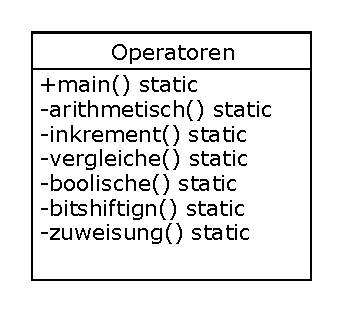
\includegraphics[width=0.45\textwidth]{uml/uml_c5_p2.pdf}
\end{center}

\subsubsection{Quelltext}
\paragraph{Operatoren.java}\
\lstinputlisting[language = Java , frame = trBL , escapeinside={(*@}{@*)}]{../chapter_05/src/main/java/chapter_05/Operatoren.java}

\subsubsection{Testdokumentation}
Es wurden alle Berechnungen korrekt ausgeführt.

\subsubsection{Benutzungshinweise}
Keine Besonderen Benutzungshinweise.
Das Programm muss lediglich nur ausgeführt werden.

\subsubsection{Anwendungsbeispiel}
Nach dem man das Programm gestartet hat, sollte folgende Ausgabe erscheinen:
\begin{lstlisting}[frame = trBL , escapeinside={(*@}{@*)}]
[sebastian@laptop bin]$ java Operatoren 
Arithmeschie Operatoren:
23 + 34 = 57
54 - 32 = 22
12 * 30 = 360
56 / 12 = 4
74 % 2  = 0
int i = +3 = 3
int n = -i = -3

Inkrement Operatoren:
x   = 10
x++ = 10
x   = 11
++x = 12
x   = 12
x-- = 12
x   = 11
--x = 10
x   = 10

Vergleichs Operatoren:
37 == 2 = false
1 != 2 = true
13 > 3 = true
23 < 2 = false
23 >= 23 = true
45 <= 44 = false

Boolische Operatoren:
!true = false
true && true = true
true || false = true
true ^ true = false

Bitweise Operatoren:
0b10111011 = ~0b01000100
0b10101010 & 0b11111111 = 10101010
0b10101010 | 0b01101001 = 10101011
0b10101010 ^ 0b11111111 = 1010101
0b10101010 >> 2 = 101010
0b10101010 >>> 1 = 1010101
0b10101010 << 1 = 101010100

Zuweisungs Operatoren:
int a = 20
a += 10 => 30
a -= 20 => 10
a *= 7 => 70
a /= 5 => 14
a %= 5 => 4
a &= 12 => 4
a |= 10 => 14
a ^= 30 => 16
a <<= 3 => 128
a >>= 1 => 64
a >>>= 2 => 16
[sebastian@laptop bin]$ 
\end{lstlisting}